\documentclass[11pt]{article}

\usepackage{a4wide}
\usepackage[utf8]{inputenc}
\usepackage[russian]{babel}
\usepackage{graphicx}
\usepackage{indentfirst} 
\usepackage{amsmath}
\usepackage{amssymb}
\usepackage{amsthm}

\begin{document}

\thispagestyle{empty}

\begin{center}
\ \vspace{-3cm}


\includegraphics[width=0.5\textwidth]{msu.eps}\\
{\scshape Московский государственный университет имени М.~В.~Ломоносова}\\
Факультет вычислительной математики и кибернетики\\
Кафедра системного анализа

\vfill

{\LARGE Отчёт по самому важному предмету}

\vspace{1cm}

{\Huge\bfseries <<Практикум в MATLAB>>}
\end{center}

\vspace{1cm}

\begin{flushright}
  \large
  \textit{Студент 315 группы}\\
  Д.\,М.~Сотников

  \vspace{5mm}

  \textit{Руководитель практикума}\\
  к.ф.-м.н., доцент П.\,А.~Точилин
\end{flushright}

\vfill

\begin{center}
Москва, 2019
\end{center}


\newpage

\section{Постановка задачи}

Для функции $f\left(\cdot\right)$ нужно найди аппроксимацию её преобразования Фурье 
при помощи быстрого преобразования Фурье и сравнить её с аналитическим решением в случае, когда
вычисление этого решения не вызывает затруднений.

Для решения поставленной задачи необходимо реализовать функцию plotFT, принимающую на вход следующие параметры:
\begin{itemize}
	\item hFigure --- handle фигуры, на которую будет осуществляться вывод графиков. 
	\item fHandle --- функция $f\left(\cdot\right)$, для которой нужно посчитать преобразование Фурье.
	\item fFTHandle --- handle функции, задающей образ Фурье функции 
	$f\left(\cdot\right)$, или $\left[\,\right]$. В последнем случае выводится только численная 
	аппроксимация.
	\item step --- шаг дискретизации.
	\item inpLimVec --- вектор $\left[a,\, b\right]$, задающий размеры окна 
	для функции $f\left(\cdot\right)$.
	\item outLimVec --- отрезок $\left[c,\, d\right]$ для вывода графика преобразования 
	Фурье. 
\end{itemize}

Протестировать корректность работы программы на следующих функциях
\begin{enumerate}
	\item $f\left(t\right) = te^{-t^2}$;
	\item $f\left(t\right) = \frac{\cos\left(t\right)-e^{-\lvert t\rvert}}{t}$;
	\item $f\left(t\right) = \frac{e^{-2\lvert t\rvert}}{1 + \cos^2\left(t\right)}$;
	\item $f\left(t\right) = \frac{2}{3+4t^4}$;
\end{enumerate}

Для первых двух вычислить их образ Фурье аналитически.

\newpage
\section{Алгоритм решения}

Для вычисления образа Фурье $F\left(\lambda\right)$ функции $f\left(\cdot\right)$, заданной на окне 
$\left[a,\ b\right]$, продолжим её на всю прямую с периодом $\left(b - a\right)$:
$$ f_0\left(x\right) = f\left(\left(x - a\right)\, \mathrm{mod} \, \left(b - a\right) + a\right),
 \quad  x \in \mathbb{R}. $$

При дискретизации функции $f$ её образ становится периодической функцией с периодом $\frac{2\pi}{\Delta}$, 
поэтому достаточно получить её значения на одном периоде.

Построим сетку $\left[-\frac{\Delta}{2},\, \left(b - a\right) 
-\frac{\Delta}{2}\right]$ размера $N$ с шагом $\Delta$ и найдем на ней значения функции $f_0$, 
то есть отсчёты  $f_0\left[n\right], \ n = 1, \ldots, N$,
к которым с помощью функции fft применим дискретное преобразование Фурье
$$ F\left[k\right] = \Delta\sum_{n=1}^{N} f\left[n\right]\exp
\left({\frac{-2\pi i \left(n-1\right)\left(k-1\right)}{N}}\right), \quad k = 1, \ldots, N. $$

Полученные отсчёты задают приближённые значения функции $F\left(\lambda\right)$ на её периоде
$\left[0,\, \frac{2\pi}{\Delta}\right]$ с шагом $\Delta_\lambda = \frac{2\pi}{b-a}$. 

Для заданного отрезка $\left[c,\, d\right]$ найдем значения образа на нём при помощи периодического 
продолжения $F\left[k\right]$. В случае, когда отрезок не задан, график выводится на симметричном 
отрезке $\left[-\frac{\pi}{\Delta},\, \frac{\pi}{\Delta}\right]$.

\newpage
\section{Вычисление преобразования Фурье некоторых функций}

В этом разделе приводятся вычисления образов Фурье первых двух функций из постановка задачи.

\begin{enumerate}
	\item
	$f(t) = te^{-t^2}$
	\begin{multline}
		F(\lambda) = \int\limits_{-\infty}^{+\infty}te^{-t^2}e^{-i\lambda t}\, dt = 
		\int\limits_{-\infty}^{+\infty}te^{-\left(t+\frac{i\lambda}{2}\right)^2 - \frac{\lambda^2}{4}}\, dt = 
		\left\{\xi = t + \frac{i\lambda}{2}\right\} = \\
		= e^{-\frac{\lambda^2}{4}}\int\limits_{-\infty}^{+\infty}\xi e^{-\xi^2}\, d\xi - 
		\frac{i\lambda}{2}e^{-\frac{-\lambda^2}{4}}\int\limits_{-\infty}^{+\infty}e^{-\xi^2}\, d\xi =
		\left\{ \text{\parbox{3cm}{функция под первым интегралом нечётна}} \right\} =-\frac{i\sqrt{\pi}\lambda}{2}e^{-\frac{\lambda^2}{4}}.
	\end{multline}
	
	\item
	$f(t) = \frac{\cos\left(t\right) - e^{-\lvert t\rvert}}{t}$
	Поскольку $f(t)$ нечётна, её образ будет чисто мнимым, и
	\begin{multline}
		F(\lambda) = -\int\limits_{-\infty}^{+\infty} f(t)\sin(\lambda t)\, dt = 
		2\int\limits_{0}^{+\infty} \frac{e^{-t} \sin\left(\lambda t\right)}{t}\, dt - 2\int\limits_{0}^{+\infty} \frac{\cos t \sin\left(\lambda t\right)}{t} \, dt = \\
		= 2\int\limits_{0}^{+\infty} \frac{e^{-t} \sin\left(\lambda t\right)}{t}\, dt - \int\limits_{0}^{+\infty} \frac{\sin\left(\left(\lambda -1\right)t\right) + \sin\left(\left(\lambda +1\right)t\right)}{t}
		\, dt = \\ = 2\int\limits_{0}^{+\infty} \frac{e^{-t} \sin\left(\lambda t\right)}{t}\, dt - \frac{\pi}{2}\left(\mathrm{sgn}\left(\lambda-1\right) + \mathrm{sgn}\left(\lambda+1\right)\right).
	\end{multline}
	
	Вычислим оставшийся интеграл $I(\lambda) = \int\limits_{0}^{+\infty} \frac{e^{-t} \sin\left(\lambda t\right)}{t}\, dt$ c помощью дифференцирования по параметру:
	\begin{multline}
	\frac{dI}{d\lambda} = \int\limits_{0}^{+\infty} e^{-t} \cos\left(\lambda t\right)\, dt = 
	-e^{-t}\cos(\lambda t)\Bigl|_0^{+\infty} - \lambda\int\limits_{0}^{+\infty} 
	e^{-t} \sin\left(\lambda t\right)\, dt =\\= -1 + e^{-t}\sin(\lambda t)\Bigl|_0^{+\infty}
	-\lambda^2 \int\limits_{0}^{+\infty} e^{-t} \cos\left(\lambda t\right)\, dt = -1 - \lambda^2\frac{dI}{d\lambda}.
	\end{multline}
	Отсюда $\frac{dI}{d\lambda} = -\frac{1}{1+\lambda^2}, \quad I = -\arctan \lambda + c$, и, так как
	$I(0) = 0$, интеграл равен 
	$$I = \frac{\pi}{2} \mathrm{sgn}\, \lambda - \arctan\lambda.$$
	а образ Фурье функции $f(t)$ имеет вид
	\begin{equation}
	F(\lambda) = 2\left(\frac{\pi}{2} \mathrm{sgn}\, \lambda - \arctan\lambda\right) -
	\frac{\pi}{2}\left(\mathrm{sgn}\left(\lambda-1\right) + \mathrm{sgn}\left(\lambda+1\right)\right).
	\end{equation}
\end{enumerate}

\newpage
\section{Визуализация результатов}
Ниже представлены графики преобразований Фурье для функций $f(t)$ из постановки задачи.
\begin{enumerate}
\item
$ f\left(t\right) = te^{-t^2} $


\noindent

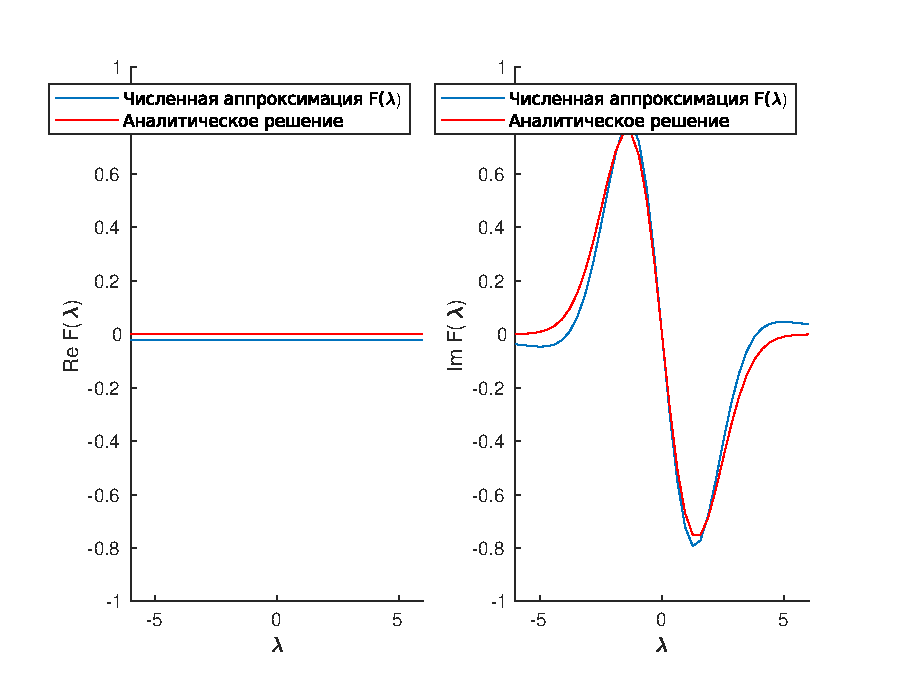
\includegraphics[width=1.0\textwidth]{gr1_2.eps}
\begin{center}
\it{рис. 1 \quad $\Delta = 0.2, \quad b = -a = 10.$}
\end{center}

Численная аппроксимация расходится с аналитическим решением из-за выбора маленького
значения  $\Delta$.

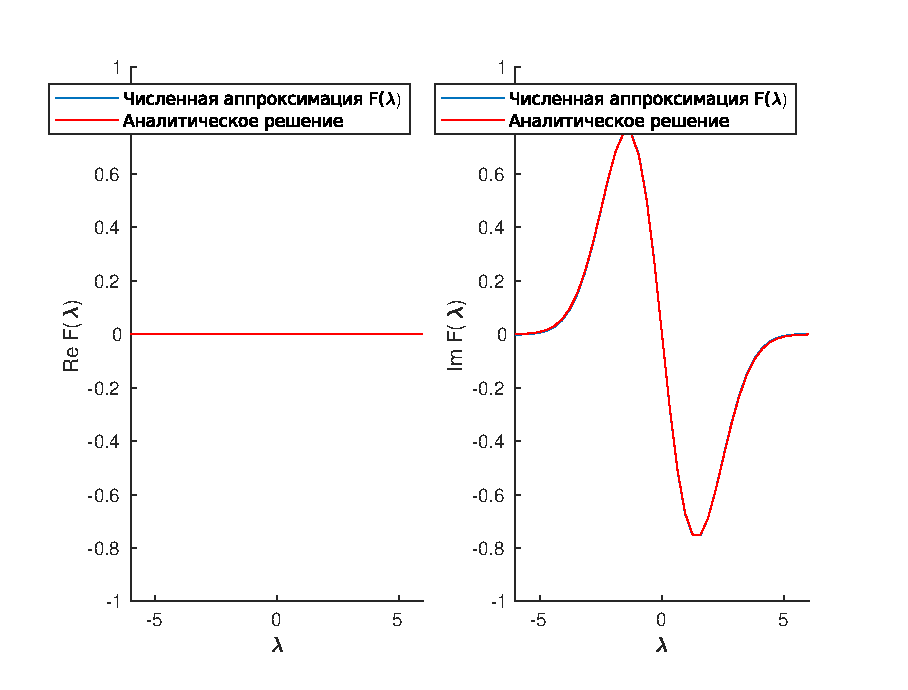
\includegraphics[width=1.0\textwidth]{gr1.eps}
\begin{center}
\it{рис. 2 \quad $\Delta = 0.01, \quad b = -a = 10.$}
\end{center}

При уменьшении $\Delta$ алгоритм дает точное приближение образа Фурье. 

\newpage
\item $f\left(t\right) = \frac{\cos\left(t\right)-e^{-\lvert t\rvert}}{t}$

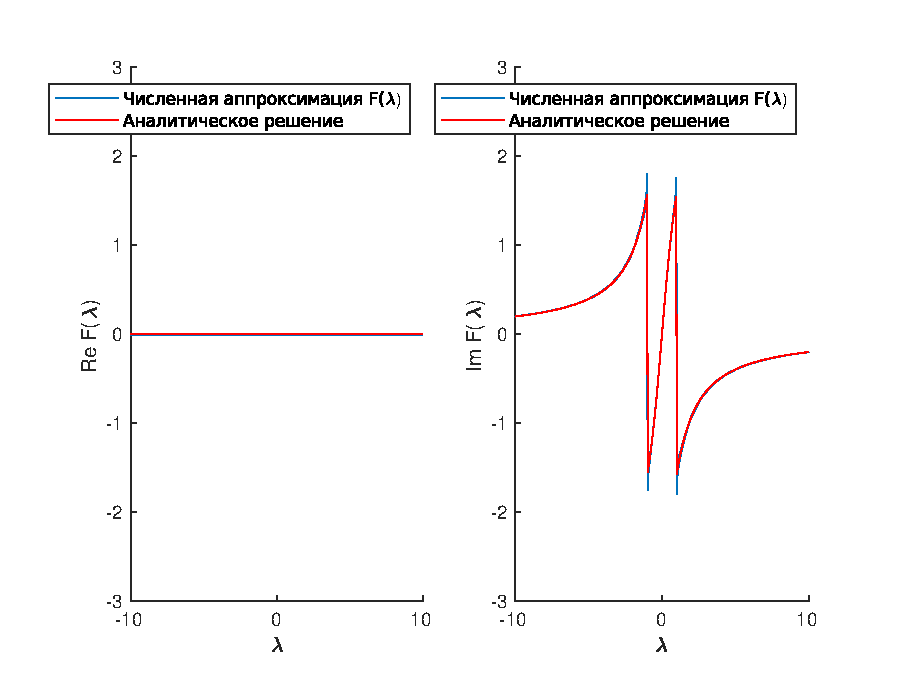
\includegraphics[width=1.0\textwidth]{gr2_1.eps}
\begin{center}
\it{рис. 3 \quad $\Delta = 0.01, \quad b = -a = 100.$}
\end{center}

При большом окне и маленькой величине шага дискретное преобразование Фурье дает точную 
аппроксимацию всюду, кроме точек разрыва функции-образа, в окрестности которой наблюдается эффект ряби.

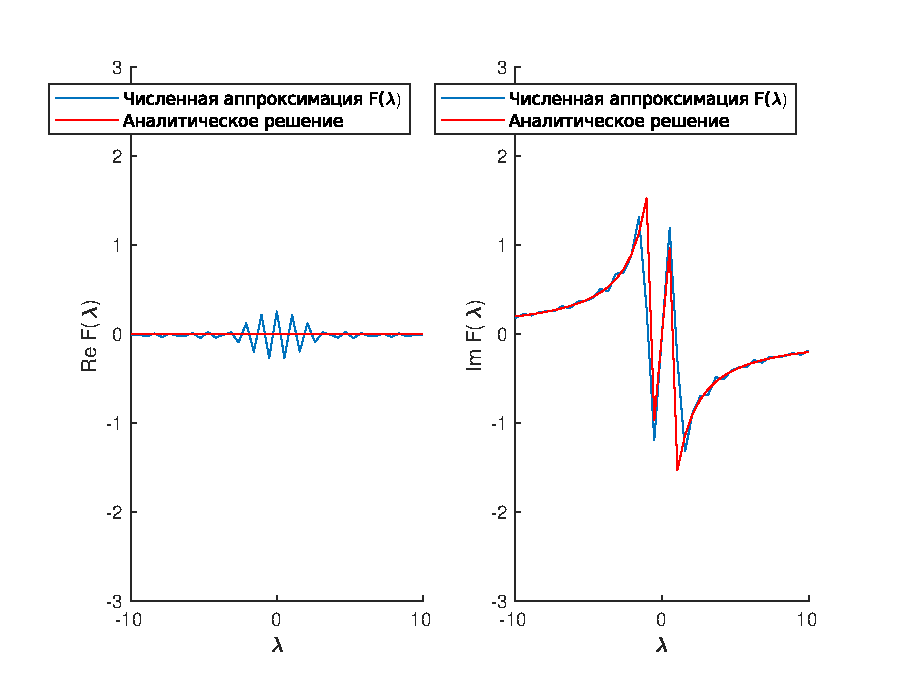
\includegraphics[width=1.0\textwidth]{gr2_2.eps}
\begin{center}
\it{рис. 4 \quad $\Delta = 0.01, \quad a = -5, \quad b = 7.$}
\end{center}

При уменьшении окна ошибка увеличивается, и появляются возмущения в вещественной части численной 
аппроксимации, связанные с несимметричностью окна.

\newpage
\item $f\left(t\right) = \frac{e^{-2\lvert t\rvert}}{1 + \cos^2\left(t\right)}$

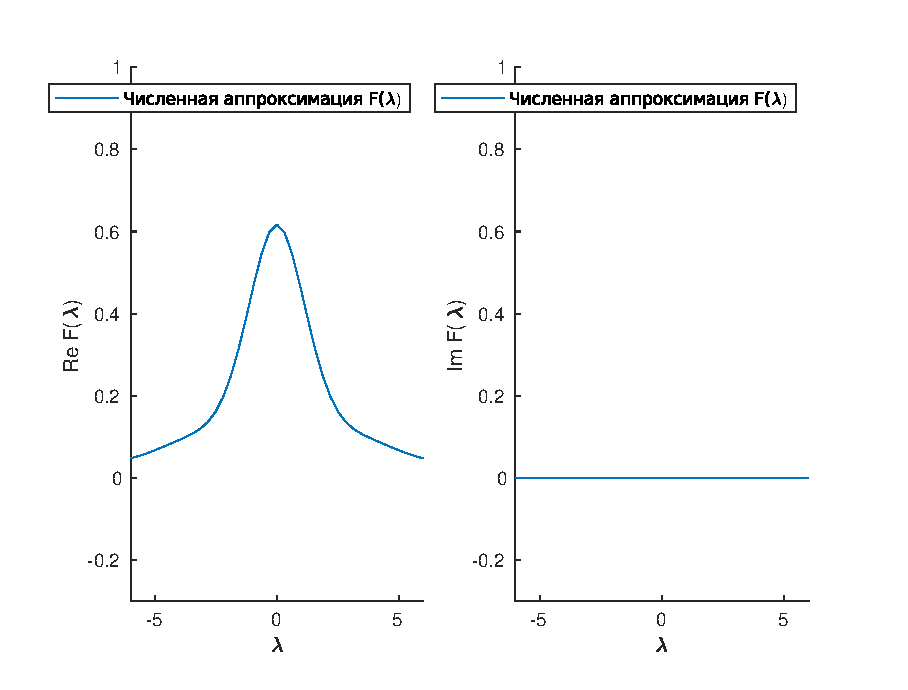
\includegraphics[width=1.0\textwidth]{gr3_1.eps}
\begin{center}
\it{рис. 5 \quad $\Delta = 0.05, \quad b = -a = 10.$}
\end{center}


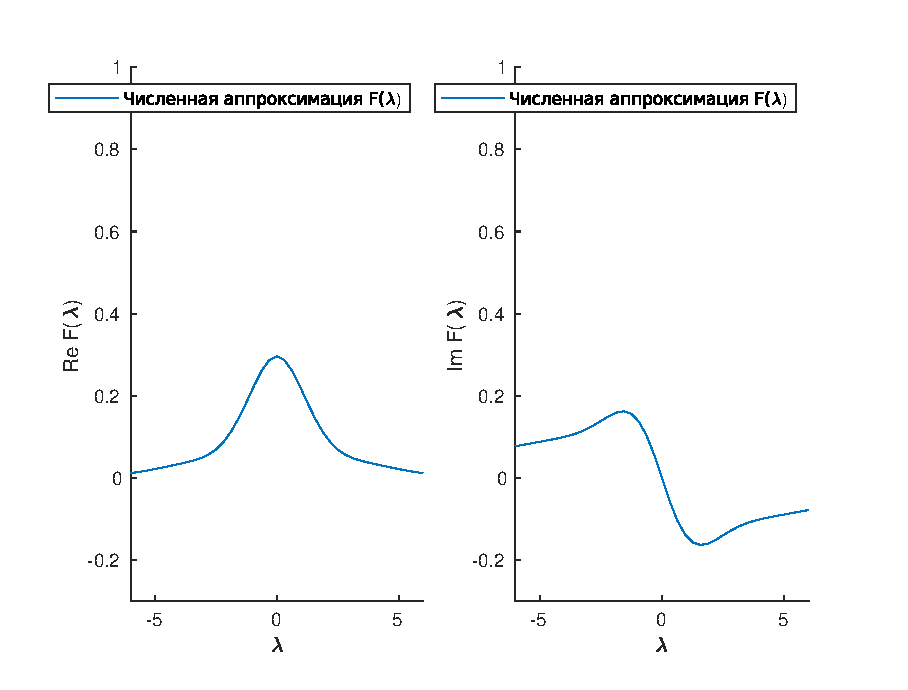
\includegraphics[width=1.0\textwidth]{gr3_2.eps}
\begin{center}
\it{рис. 6 \quad $\Delta = 0.05, \quad a = 0, \quad b = 20.$}
\end{center}

В силу выбора нессиметричного окна функция образа перестает быть чисто мнимой.

\newpage
\item $f\left(t\right) = \frac{2}{3+4t^4}$

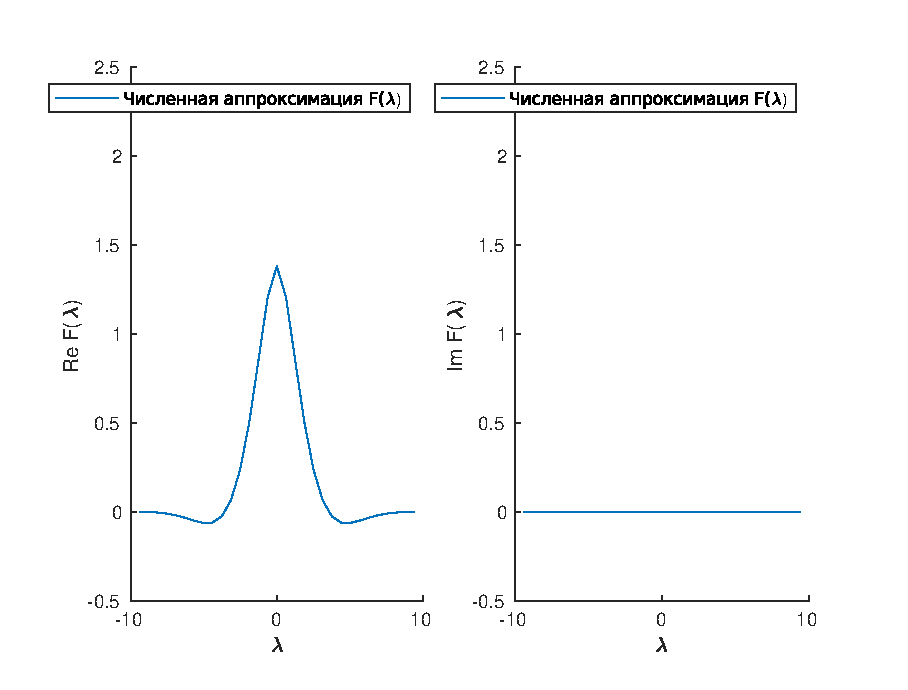
\includegraphics[width=1.0\textwidth]{gr4_1.eps}
\begin{center}
\it{рис. 7 \quad $\Delta = 0.01, \quad b = -a = 5.$}
\end{center}

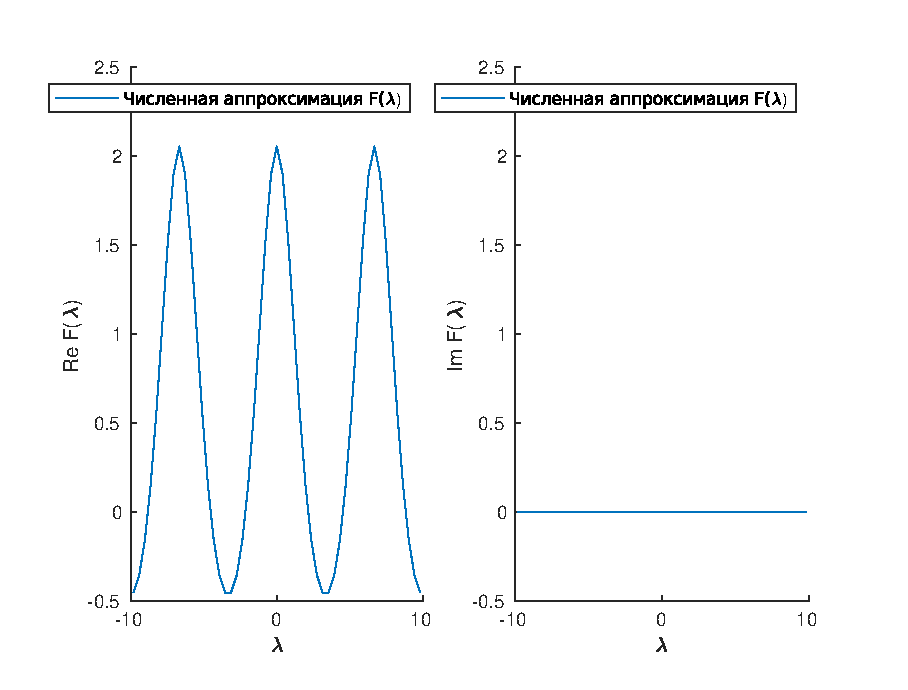
\includegraphics[width=1.0\textwidth]{gr4_2.eps}
\begin{center}
\it{рис. 8 \quad $\Delta = 1, \quad b = -a = 8.$}
\end{center}

Из-за выбора большого шага дискретизации уменьшается период образа.
\end{enumerate}

\newpage
\section{Эффект наложения спектра}
Пример наложения спектра для образа Фурье функции $ f\left(t\right) = te^{-t^2} $.
При больших размерах окна ($b - a = 14$) существенного наложения не происходит. При уменьшении 
размеров окна появляется наложение, и сумма образов портится. 

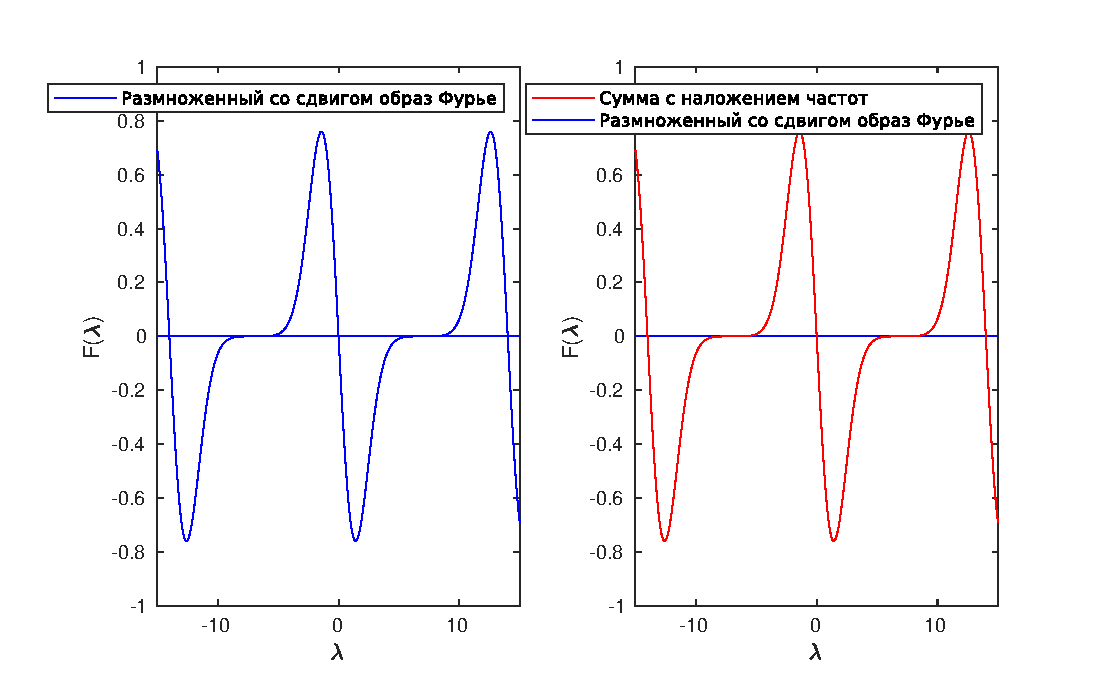
\includegraphics[width=1.0\textwidth]{aliasing1.eps}
\begin{center}
\it{рис. 9 \quad $b - a = 14$}
\end{center}

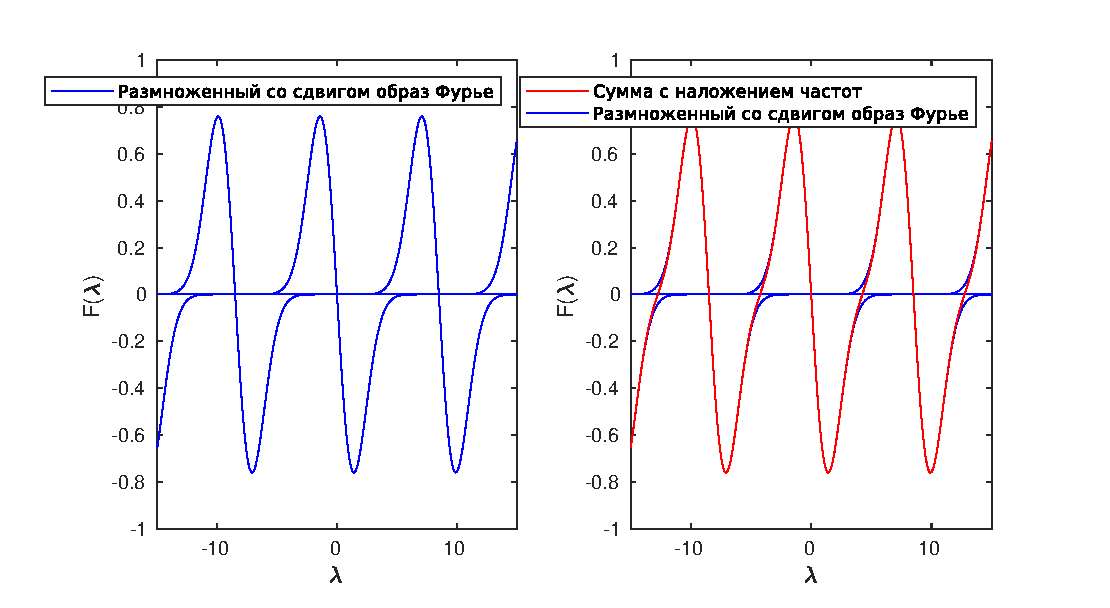
\includegraphics[width=1.0\textwidth]{aliasing2.eps}
\begin{center}
\it{рис. 10 \quad $b - a = 8.5$}
\end{center}


\newpage
\section{Эффект ряби}
Эффект ряби можно продемонстрировать на примере функции 
$f\left(t\right) = \frac{\cos\left(t\right)-e^{-\lvert t\rvert}}{t}$, образ Фурье которой
является разрывной функцией.

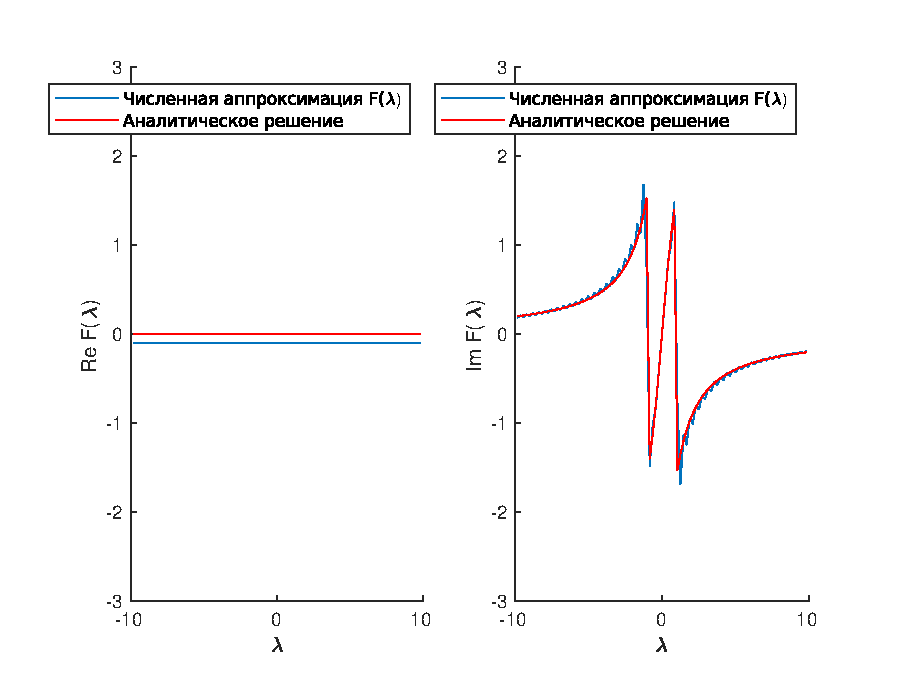
\includegraphics[width=1.0\textwidth]{ripple_1.eps}
\begin{center}
\it{рис. 11 \quad $\Delta = 0.1, \quad b = -a = 15.$}
\end{center}

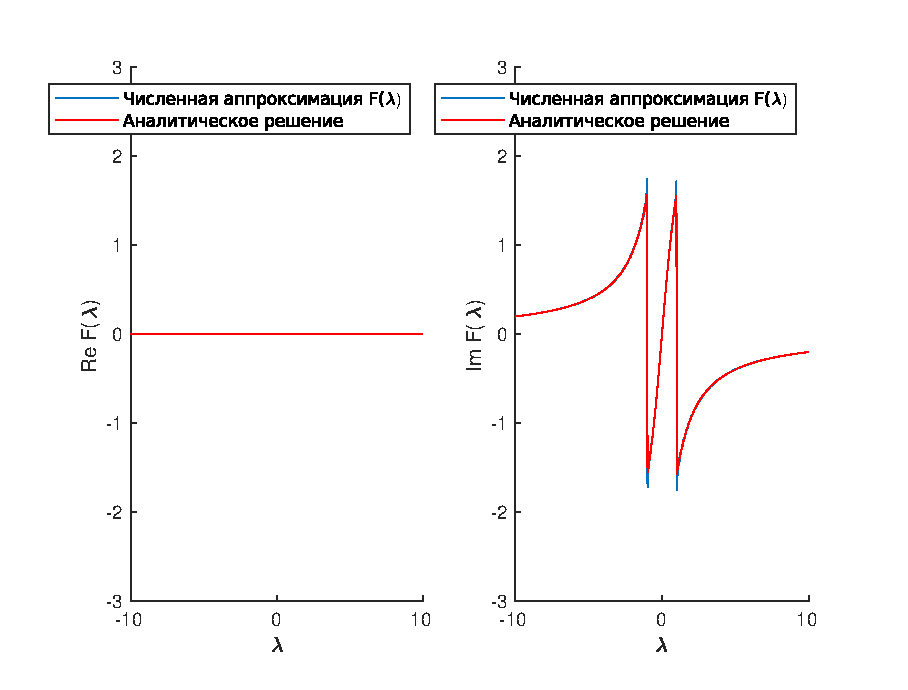
\includegraphics[width=1.0\textwidth]{ripple_2.eps}
\begin{center}
\it{рис. 12 \quad $\Delta = 0.001, \quad b = -a = 150.$}
\end{center}

На множестве непрерывности фукнции-образа от ряби можно избавиться, уменьшив шаг дискретизации и
увеличив размер окна. Однако устранить рябь вблизи точки разрыва функции $F(\lambda)$ невозможно.
\end{document}